\documentclass[12pt]{article}
\usepackage{amssymb, amsmath, hyperref}
\DeclareMathAlphabet{\mathscr}{OT1}{pzc}{m}{it}
\usepackage{epsfig, graphicx}
\usepackage{verbatim}
\usepackage{fullpage,setspace}
\title{Photon-Bunching in Quantum Memory}
\author{Adam A. G. Green\\Univeristy of Calgary}
\begin{document}
\bibliographystyle{plain}
\maketitle
\section{Introduction}
\doublespacing
\section{Demonstration}

Any quantum memory that has the `beamplitter' like hamiltonian will show this:
\begin{equation}
H_{\textrm{int}}= J^* a^\dagger b + J a b^\dagger
\end{equation}

where $a$ and $b$ obey bosonic communtation relations. On a higher level, this is a function of photon bunching, but there are several inherent limitations and interesting cases when a quantum memory is applied.

\section{CD Memory}
We can demonstrate photon bunching explicitly in the case of the CD memory\cite{arxiv}. This quantum memory is used because the author was familiar with the equations of motion.

We have previously derived the heisenburg equations of motion for the operators of interest, $E_{\textrm{out}}$ and $\sigma_{\textrm{z?}}$.

The heisenburg state we prepared for photon bunching is:
\begin{equation}
| \psi \rangle = \sigma(t=0)^\dagger \int d\omega \psi(w) E_0^\dagger(w) | 0 \rangle
\end{equation}

Where $E_0(\omega)$ is the creation operator of a photon of frequency $\omega$, $\psi(\omega)$ is the single-photon envelope in frequency space, and $\sigma(t=0)$ is the initial creation operator of a atomic excitation. In what follows, we will be assuming that a photon is already stored in the memory at $t=0$, and that another pulse is incident.

The three terms we are concered with are:
\begin{align}
\langle \psi_{20}| \Psi \rangle &=\langle 0 | \frac{1}{\sqrt{2}}\sigma \sigma | \Psi \rangle\\
\langle \psi_{11} | \Psi \rangle& =\langle 0 |  \sigma(t') \int^{t'} dt E_\textrm{out}(t) | \Psi \rangle\\
\langle \psi_{02} | \Psi \rangle &= \langle 0 |  \frac{1}{\sqrt{2}}\int dt \int dt' E_\textrm{out}(t) E_\textrm{out}(t') | \Psi \rangle
\end{align}

Where $| \psi_{20}$ is a double excitation in the photon field, $| \psi_{11} \rangle $ is photon and an atomic excitation, and $ | \psi_{02} \rangle $ is a double atomic excitation. 
\section{$| \psi_{11} \rangle$}
First, we consider the term that deals with a single excitation in the field and a single
excitation in the atom. If photon-bunching is seen in this memory, then this term should
equal zero.

\begin{align}
\left | \langle \psi_{11} | \Phi \rangle \right | ^2 &=\int^{t'} dt \left | \langle 0 | E_\textrm{out}(t) \sigma(t') \int d \omega \phi(\omega)E^\dagger_0(\omega)
\sigma^\dagger(0) | 0 \rangle \right |^2 \\
\end{align}


We also know the equations for $E_\text{out} (t)$ and $\sigma (t)$ from our previous work.

\begin{equation}
E_\textrm{out}(t) = E_\textrm{in}(t) + i \sqrt{\frac{2}{\kappa}} g(t) \sigma(t)\\
\sigma(t) = \sigma(0) e^{-\tau} + i\sqrt{2} e^{-\tau} \int^\tau_w d t' e^\tau E_\textrm{in}(t) \frac{g(t)}{\sqrt{\kappa}}
\end{equation}
Where $\tau = \int^t dt g^2(t)/\kappa$, $g(t)$ is a time-dependant coupling between the atomic ensemble and the cavity field, and $\kappa$ is the decay rate of the cavity. Inserting these equations we obtain:
Inserting these gives:
\begin{align}
\left | \langle \psi_{11} | \Phi \rangle \right | ^2 &= \int^{t'} dt \left | \langle 0 |
   \left(  E_\textrm{in}(t) + i \sqrt{\frac{2}{\kappa}} g(t) \sigma(t) \right ) \times \right.\\
   &\left. \qquad \qquad \left (\sigma(0) e^{-\tau} + i\sqrt{2} e^{-\tau} \int^\tau_w d t' e^\tau E_\textrm{in}(t) \frac{g(t)}{\sqrt{\kappa}}\right)|\Psi \rangle \right |^2\\
\end{align}

Expanding this out, we get the following terms:
\begin{align}
\left | \langle \psi_{11} | \Phi \rangle \right | ^2 &= 
\int^{t'} dt \left | \langle 0 | E_\textrm{in}(t) \left( \sigma(0) e^{-\tau(t')} + i\sqrt{2} e^{-\tau(t')} \int^{t'} d t'' e^{\tau(t'')} E_\textrm{in}(t'') \frac{g(t'')}{\sqrt{\kappa}} \right )\right. \\
&\qquad+ i \sqrt{\frac{2}{\kappa}}g(t)\left (\sigma(0) e^{-\tau} + i\sqrt{2} e^{-\tau} \int^{t}d t''' e^{\tau(t''')} E_\textrm{in}(t''') \frac{g(t''')}{\sqrt{\kappa}} \right) \times\\
&\left.\qquad \left(\sigma(0) e^{-\tau(t')} + i\sqrt{2} e^{-\tau(t')} \int^{t'} d t'' e^\tau(t'') E_\textrm{in}(t'') \frac{g(t'')}{\sqrt{\kappa}}\right) | \Psi \rangle \right |^2 
\end{align}

If we apply the commutation relations, we can get rid of any terms that don't have $E_\textrm{in}(t)$ and $\sigma(0)$ in them, as any term in the above equation that doesn't have both of these operators will be anhilated through simple commutations. Ie. if a term only has $E_\textrm{in} E_\textrm{in}$, we know that $|\Psi\rangle$ contains a $\sigma^\dagger(0)$, and that $\sigma^\dagger(0)$ and $E_\textrm{in}$ commute, so $\sigma^\dagger(0)$ can move through and act as $\langle 0 | \sigma^\dagger(0) = 0$. So any term that survives must contain terms that don't commute with $E_\textrm{in}$ as well as $\sigma(0)$.

This leaves us with the following terms:
\begin{align}
\left | \langle \psi_{11} | \Phi \rangle \right | ^2 &= \int^{t'} dt \left | \langle 0 | E_\textrm{in}(t) \sigma(0) e^{-\tau(t')}
\sigma^\dagger(0) \int d\omega E_0(\omega) \phi(\omega) | 0 \rangle -\right. \\
&\qquad  \langle 0 | \frac{2}{\sqrt{\kappa}} g(t) \sigma(0) e^{-\tau(t) -\tau(t')}
\int^{t'} dt'' e^{\tau(t'')} E_\textrm{in}(t'')\frac{g(t'')}{\sqrt{\kappa}} \sigma^\dagger(0) \int d\omega E_0(\omega) \phi(\omega) | 0 \rangle - \\
& \qquad \left. \langle 0 | \frac{2}{\sqrt{\kappa}} g(t) \sigma(0) e^{-\tau(t) -\tau(t')}
\int^{t} dt''' e^{\tau(t''')} E_\textrm{in}(t''')\frac{g(t''')}{\sqrt{\kappa}} \sigma^\dagger(0) \int d\omega E_0(\omega) \phi(\omega) | 0 \rangle \right |^2
\end{align}


We know that $E_\textrm{in}$ is the input-pulse, and can also be defined in frequency space as $E_\textrm{in} = \int dw e^{-iwt} E_0(\omega) $ and furthermore, $[E_0(\omega), E_0^\dagger(\omega') ] = \delta(\omega-\omega')$, thus we know that 

\begin{align}
\langle 0 |E_\textrm{in}(t) \int d\omega E^\dagger_0(\omega) | 0 \rangle= \mathscr{F}\{\phi(\omega)\} \equiv \tilde{\phi}(t)
\end{align}

using this property, the equation reduces to:
%As well, if we make the simplifying assumption that $\tilde{\phi}(t) = \sqrt{\frac{2}{\kappa}} g(t)e^{\tau(t)}$, then %the equation reduces to:

\begin{align}
\left | \langle \psi_{11} | \Phi \rangle \right | ^2 &= \int^{t'} dt\left| \tilde{\phi}(t)e^{-\tau(t')} -\frac{2}{\sqrt{\kappa}} g(t) e^{-\tau(t)-\tau(t')} \int^{t'} \tilde{\phi}(t'')\frac{g(t'')}{\sqrt{\kappa}} dt'' - \right.\\
&\left. \qquad \frac{2}{\sqrt{\kappa}} g(t) e^{-\tau(t)-\tau(t')} \int^t \tilde{\phi}(t''')\frac{g(t''')}{\sqrt{\kappa}} dt''' \right |^2 
\end{align}

Note, we haven't shown how the $\sigma(0) \sigma^\dagger(0)$ term vanishes, but using the communtator properties, you can show that in this case you can simply replace this term with unity.

This is a completely general equation, as we have not assumed anything about the shape of the incoming field. 
To simply this equation however, we can make the assumption that the incoming field meets the optimal condition discussed
in the original paper.

This allows us to do two things. First, because the field is optimally conditioned, all of the efficiency is controlled by the value of $\tau_w$, so we only have one variable to deal with. Second, it will allow the above equation to be integrated very simply.

The optimal condition requires that: $\tilde{\phi}(t) = \sqrt{\frac{2}{\kappa}} g(t) e^{\tau(t)}$
Inserting this into our equation, we obtain:

\begin{align}
\left | \langle \psi_{11} | \Phi \rangle \right | ^2 &= \int^{t'} dt \left | \sqrt{\frac{2}{\kappa}} g(t) e^{\tau(t)-\tau(t')} \right.
      -2\sqrt{\frac{2}{\kappa}}g(t) e^{-\tau(t)-\tau(t')} \int^{t'} \frac{g(t'')^2}{\kappa} e^{2\tau(t'')} dt'' \\
       &\qquad \left.-2\sqrt{\frac{2}{\kappa}} g(t) e^{\tau(t')-\tau(t)} \int^t \frac{g(t''')^2}{\kappa} e^{2\tau(t''')} dt'''\right |^2
\end{align}

and, knowing that $\frac{g^2(t)}{\kappa}dt = d\tau$, the above can be integrate to obtain:

\begin{align}
\left | \langle \psi_{11} | \Phi \rangle \right | ^2 &=\int^{t'} dt \left| \sqrt{\frac{2}{\kappa}} g(t) e^{\tau(t)-\tau(t')} - \sqrt{\frac{2}{\kappa}} g(t)\left( e^{\tau(t)-\tau(t')} - e^{-\tau(t')-\tau(t)} \right )\right.\\
&\left. \qquad -\sqrt{\frac{2}{\kappa}} g(t) \left( e^{\tau(t')-\tau(t)} - e^{-\tau(t')-\tau(t)} \right)\right|^2 
\end{align}

which can be factored to obtain:
\begin{align}
\left | \langle \psi_{11} | \Phi \rangle \right | ^2  &= \int^{t'} dt \left|\sqrt{\frac{2}{\kappa}} g(t) e^{-\tau(t)} \left (- e^{\tau(t')} +2 e^{-\tau(t')} \right ) \right |^2 
\end{align}

If use the condition that $\eta=0.5$, then $\tau(t') = \textrm{ln}(\sqrt{2})$. It should be noted that $\tau(t=\infty) = \tau(t')$. That is, we have let an infinite time pass when we do the measurment. We are preforming a measurement on the atomic ensemble at time $t'$, but we have left out photon decectors on from time $t_0$ to $t'$. However, because we know what $\tau(t')$ is equal to, we can evaluate the term in brackets in the above equation.

\begin{align}
\left | \langle \psi_{11} | \Phi \rangle \right | ^2 = \int^{t'} dt \left| \sqrt{\frac{2}{\kappa}} g(t) e^{-\tau(t)} \left ( e^{\textrm{ln}(\sqrt{2})} -2 \frac{1}{e^{\textrm{ln}({\sqrt{2}})}} \right ) \right|^2 = 0 
\end{align}

This shows that there is zero chance to measure a photon in the reserviour field and an atomic excitation when the quantum is oppurtating at $50\%$ efficieny. This is precisely what is expected for a beam-splitter.


\section{ $| \psi_{20} \rangle$}
Next, we deal with the case term that measures the amplitude of obtaining a double excitation in the atomic ensemble.
\begin{align}
\langle \phi_{20}| \Psi \rangle &=\langle 0 |\frac{1}{\sqrt{2}} \sigma \sigma | \Psi \rangle\\
\langle \phi_{20}| \Psi \rangle &=\langle 0 | \frac{1}{\sqrt{2}} \sigma \sigma 
\sigma(t=0)^\dagger \int d\omega \psi(w) E_0^\dagger(w) | 0 \rangle
\end{align}

and the heisenburg equations for the operators $E_\textrm{out}$ and $\sigma$ are:
\begin{equation}
E_\textrm{out}(t) = E_\textrm{in}(t) + i \sqrt{\frac{2}{\kappa}} g(t) \sigma(t) \\
\sigma(t) = \sigma(0) e^{-\tau} + i\sqrt{2} e^{-\tau} \int^\tau_w d t' e^\tau E_\textrm{in}(t) \frac{g(t)}{\sqrt{\kappa}}
\end{equation}
Where $\tau = \int^t dt g^2(t)/\kappa$, $g(t)$ is a time-dependant coupling between the atomic ensemble and the cavity field, and $\kappa$ is the decay rate of the cavity. Inserting these equations we obtain:
\begin{multline}
\langle \phi_{20}| \Psi \rangle =\langle 0 | \frac{1}{\sqrt{2}} \left (  \sigma(0) e^{-\tau} + i\sqrt{2} e^{-\tau} \int^\tau_w d t' e^\tau E_\textrm{in}(t) \frac{g(t)}{\sqrt{\kappa}} \right )\\ \left ( \sigma(0) e^{-\tau} + i\sqrt{2} e^{-\tau} \int^\tau_w d t' e^\tau E_\textrm{in}(t) \frac{g(t)}{\sqrt{\kappa}} \right ) \sigma(t=0)^\dagger \int d\omega \psi(w) E_0^\dagger(w) | 0 \rangle
\end{multline}
As shown before, we know the following relation,
\begin{equation}
E_\textrm{in} \int dw' \phi(\omega') E_0^\dagger(\omega') = \mathscr{F}[\phi(\omega)]
\end{equation}

And we know that the only terms that will survive in $\langle \phi |$ must contain $E_\textrm{in}(t) sigma(t)$. This leaves the following expansion:
\begin{align}
\langle \psi_{20}| \Psi \rangle &= 2 i e^{-2\tau} \sigma(0) 
\int^{\tau'} E_{in}(\tau') \frac{g(\tau')}{\sqrt{\kappa}} e^{\tau'} \sigma^\dagger(0) \int dw' E_0(\omega') \psi(\omega')\\ 
&= 2 i e^{-2 \tau} \int d \tau' e^{\tau'} 
 \mathscr{F}(\psi(\omega)) \frac{\sqrt{\kappa}}{g(\tau')}
\end{align}

Now, we can also make a simplifying assumption, by noting that the optimal read-in condition is met when $\mathscr{F}(\psi(\omega)) = \sqrt{\frac{2}{\kappa}} g(t) e^{\tau(t)}$ and under this condition is met, the above equation reduces to:
\begin{align}
\langle \psi_{20}| \Psi \rangle & = 2\sqrt{2} i e^{-2\tau} \int d \tau' e^{2 \tau} \\
& = \sqrt{2} i\left(1- e^{-2\tau}\right)
\end{align}

Also, as previously shown, we know that $\tau$ is equal to $\tau_w = \ln{\sqrt{2}}$, so we can evaluate the above equation to obtain:
\begin{align}
\langle \psi_{20}| \Psi \rangle &= \sqrt{2} i \frac{1}{2} \\
&= \frac{i}{\sqrt{2}}
\end{align}

Now, to obtain the probability, we square this to obtain:
\begin{equation}
| \langle \psi_{20}| \Psi \rangle | ^2 = \frac{1}{2}
\end{equation}
\section{$| \psi_{02} \rangle $}

We could invoke a conservation of probability to show that since this is the only other state that is possible in the double excitation space, it must have probability $1/2$, however it is good to do the calculations out to double check.

The quantity that we are interested in is the probability of measuring a double excitation in the reserviour field:

\begin{align}
|\langle \psi_{02} | \Psi \rangle |^2 =\int dt \int dt' \left | \langle 0 |\frac{1}{\sqrt{2}} E_\textrm{out}(t) E_\textrm{out}(t') \sigma^\dagger(0) \int d \omega \phi(\omega) E_0(\omega) | 0 \rangle \right |^2
\end{align}

Using the equations for $E_\textrm{out}(t)$, this becomes:
\begin{align}
\left | \langle \psi_{02} | \Phi \rangle \right | ^2 & =\int dt \int dt'\left |  \frac{1}{\sqrt{2}}\left ( E_\textrm{in}(t) 
+ i \sqrt{\frac{2}{\kappa}} g(t)\left ( \sigma(0) e^{-\tau} +
i\sqrt{2} e^{-\tau} \int^t d t''' e^\tau(t''') E_\textrm{in}(t''') \frac{g(t''')}{\sqrt{\kappa}} \right ) \right) \right .\times \\
 &\qquad \left. \left (E_\textrm{in}(t') + i \sqrt{\frac{2}{\kappa}} g(t')\left( \sigma(0) e^{-\tau(t')} +
 i\sqrt{2} e^{-\tau(t')} \int^{t'} d t'' e^\tau(t'') E_\textrm{in}(t'') \frac{g(t'')}{\sqrt{\kappa}}\right ) \right ) \right | \Psi \rangle |^2
\end{align}

 
 As before, we know that only terms that contain $E_\textrm{in}$ and $\sigma(0)$ will survive the expansion. With this in 
 mind, we can reduce the above equation to:
\begin{align}
 \left | \langle \psi_{02} | \Phi \rangle \right | ^2 & = \frac{1}{2}\int dt \int dt'\left |\langle 0 | E_\textrm{in}(t) i \sqrt{\frac{2}{\kappa}} g(t') e^{-\tau(t')}\sigma(0) + E_\textrm{in}(t') i \sqrt{\frac{2}{\kappa}} g(t) e^{-\tau(t)}\sigma(0) +\right.\\
&\qquad -i\sqrt{2}\frac{2}{\sqrt{\kappa}}g(t')g(t) e^{-\tau(t')-\tau(t)}\sigma(0) \int ^{t'} dt'' E_\textrm{in}(t'')\frac{g(t'')}{\sqrt{\kappa}} e^{\tau(t'')}\\
&\qquad \left. -i\sqrt{2}\frac{2}{\sqrt{\kappa}}g(t')g(t) e^{-\tau(t')-\tau(t)}\sigma(0) \int ^t dt''' E_\textrm{in}(t''')\frac{g(t''')}{\sqrt{\kappa}} e^{\tau(t''')}| \Psi \rangle\right| \Psi \rangle |^2
 \end{align}
 
Again, knowing that


\begin{align}
\langle 0 |E_\textrm{in}(t) \int d\omega E^\dagger_0(\omega) | 0 \rangle= \mathscr{F}\{\phi(\omega)\} \equiv \tilde{\phi}(t)
\end{align}
and again using the optimization condtion: $\tilde{\phi}(t) = \sqrt{\frac{2}{\kappa}} g(t) e^{\tau}$, we can obtain the following equation:

\begin{align}
\left | \langle \psi_{02} | \Phi \rangle \right | ^2 & = \frac{1}{2}\int dt \int dt'\left | \frac{2}{\kappa} i g(t) g(t') \left(e^{\tau-\tau'} +e^{-(\tau-\tau')}\right) -\right.\\
&\qquad \left.i \frac{4}{\kappa}g(t) g(t') e^{-\tau-\tau(t')}\left( \int^{t'} d \tau(t'') e^{2\tau(t'')} - \int^t d \tau(t''') e^{2\tau(t''')} \right) \right |^2
\end{align}

Integrating this, we obtain:
\begin{align}
\left | \langle \psi_{02} | \Phi \rangle \right | ^2 & = \frac{1}{2}\int dt \int dt'\left | \frac{2}{\kappa} i g(t) g(t') \left(e^{\tau-\tau'} +e^{-(\tau-\tau')}\right) -\right.\\
&\qquad \left.i \frac{2}{\kappa}g(t) g(t') e^{-\tau-\tau(t')}\left( e^{2\tau(t')}-1 - e^{2\tau(t)}-1 \right) \right |^2 \\
 &=  \frac{1}{2}\int dt \int dt'\left | \frac{2}{\kappa} i g(t) g(t') \left(e^{\tau-\tau'} +e^{-(\tau-\tau')}\right) +\right.\\
&\qquad \left.i \frac{2}{\kappa}g(t) g(t') \left( e^{\tau(t')-\tau(t)} + e^{\tau(t)-\tau(t')}-2e^{-\tau(t)-\tau(t')} \right) \right |^2
\end{align}

There is some cancellation, leaving:

\begin{align}
\left | \langle \psi_{02} | \Phi \rangle \right | ^2 & =\int dt \int dt'\left |i 2\frac{\sqrt{2}}{\kappa} g(t)g(t') e^{-\tau(t)-\tau(t')} \right|^2 \\
&= \frac{8}{4} \left ( e^{-2\tau_w}-1\right)^2\\
\end{align}

Now, if we require that $\tau_w = \textrm{ln}(\sqrt{2})$, this further reduces to:
\begin{align}
\left | \langle \psi_{02} | \Phi \rangle \right | ^2 &=2(-\frac{1}{2})(-\frac{1}{2})=\frac{1}{2}
\end{align}

\section{Interpretation Problems}
The following graph highlights the recent interpration problem I have found.
\begin{figure}
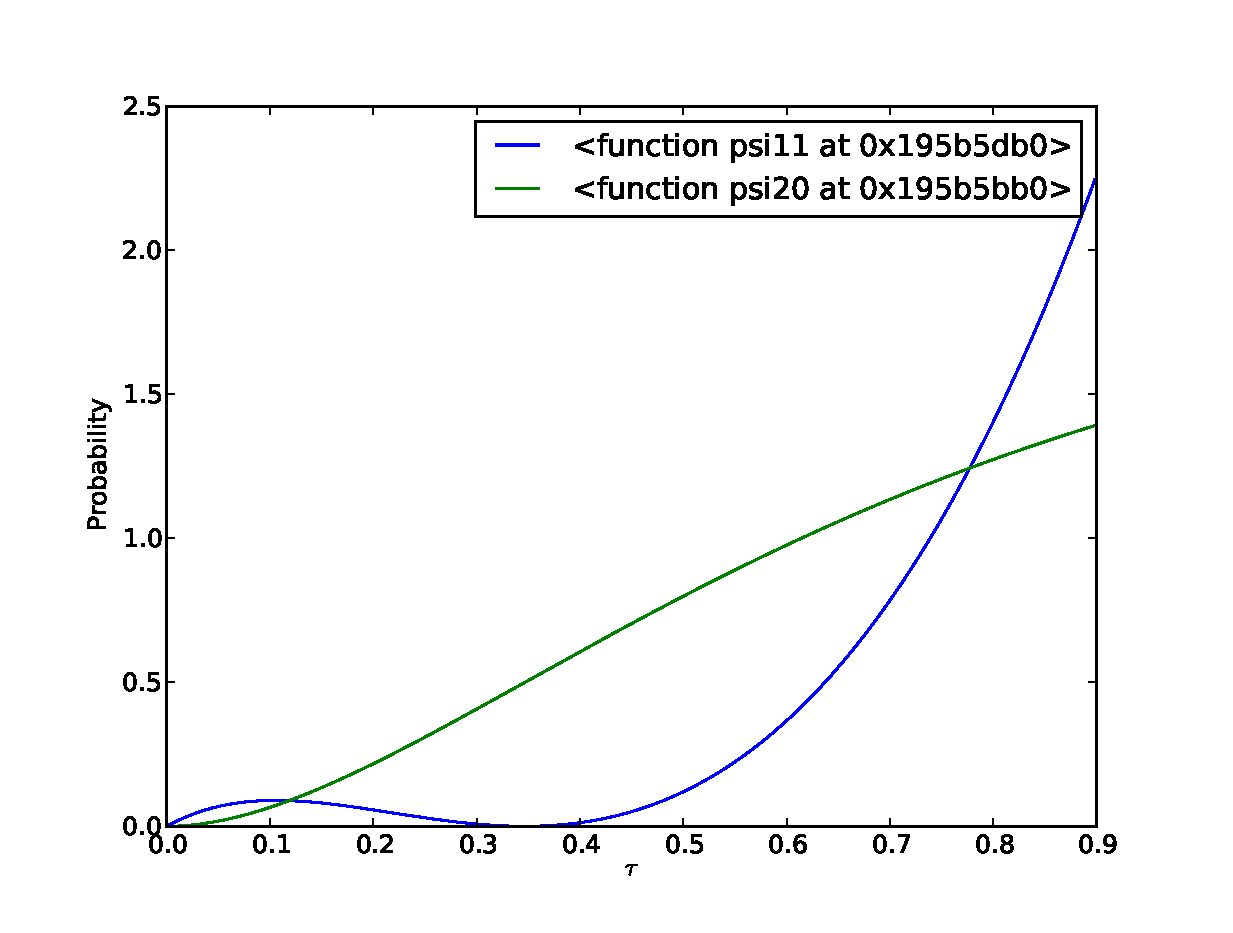
\epsfig{file=probgraph.eps,width=1. \columnwidth}
\caption{This illustrates the problem. The functions $| \langle \psi_{11}|\Psi\rangle|^2$ and $\langle \psi_{20}|\Psi\rangle|^2$ are plotted. Note:$\langle \psi_{20}|\Psi\rangle|^2=\langle \psi_{02}|\Psi\rangle|^2$. As calculated, the probability adds up to one for $\tau_w = \ln(\sqrt{2})$ but no other. \label{levels}}
\end{figure}


\end{document}
